% Options for packages loaded elsewhere
% Options for packages loaded elsewhere
\PassOptionsToPackage{unicode}{hyperref}
\PassOptionsToPackage{hyphens}{url}
\PassOptionsToPackage{dvipsnames,svgnames,x11names}{xcolor}
%
\documentclass[
]{article}
\usepackage{xcolor}
\usepackage[margin=1in]{geometry}
\usepackage{amsmath,amssymb}
\setcounter{secnumdepth}{5}
\usepackage{iftex}
\ifPDFTeX
  \usepackage[T1]{fontenc}
  \usepackage[utf8]{inputenc}
  \usepackage{textcomp} % provide euro and other symbols
\else % if luatex or xetex
  \usepackage{unicode-math} % this also loads fontspec
  \defaultfontfeatures{Scale=MatchLowercase}
  \defaultfontfeatures[\rmfamily]{Ligatures=TeX,Scale=1}
\fi
\usepackage{lmodern}
\ifPDFTeX\else
  % xetex/luatex font selection
\fi
% Use upquote if available, for straight quotes in verbatim environments
\IfFileExists{upquote.sty}{\usepackage{upquote}}{}
\IfFileExists{microtype.sty}{% use microtype if available
  \usepackage[]{microtype}
  \UseMicrotypeSet[protrusion]{basicmath} % disable protrusion for tt fonts
}{}
\makeatletter
\@ifundefined{KOMAClassName}{% if non-KOMA class
  \IfFileExists{parskip.sty}{%
    \usepackage{parskip}
  }{% else
    \setlength{\parindent}{0pt}
    \setlength{\parskip}{6pt plus 2pt minus 1pt}}
}{% if KOMA class
  \KOMAoptions{parskip=half}}
\makeatother
% Make \paragraph and \subparagraph free-standing
\makeatletter
\ifx\paragraph\undefined\else
  \let\oldparagraph\paragraph
  \renewcommand{\paragraph}{
    \@ifstar
      \xxxParagraphStar
      \xxxParagraphNoStar
  }
  \newcommand{\xxxParagraphStar}[1]{\oldparagraph*{#1}\mbox{}}
  \newcommand{\xxxParagraphNoStar}[1]{\oldparagraph{#1}\mbox{}}
\fi
\ifx\subparagraph\undefined\else
  \let\oldsubparagraph\subparagraph
  \renewcommand{\subparagraph}{
    \@ifstar
      \xxxSubParagraphStar
      \xxxSubParagraphNoStar
  }
  \newcommand{\xxxSubParagraphStar}[1]{\oldsubparagraph*{#1}\mbox{}}
  \newcommand{\xxxSubParagraphNoStar}[1]{\oldsubparagraph{#1}\mbox{}}
\fi
\makeatother


\usepackage{longtable,booktabs,array}
\usepackage{calc} % for calculating minipage widths
% Correct order of tables after \paragraph or \subparagraph
\usepackage{etoolbox}
\makeatletter
\patchcmd\longtable{\par}{\if@noskipsec\mbox{}\fi\par}{}{}
\makeatother
% Allow footnotes in longtable head/foot
\IfFileExists{footnotehyper.sty}{\usepackage{footnotehyper}}{\usepackage{footnote}}
\makesavenoteenv{longtable}
\usepackage{graphicx}
\makeatletter
\newsavebox\pandoc@box
\newcommand*\pandocbounded[1]{% scales image to fit in text height/width
  \sbox\pandoc@box{#1}%
  \Gscale@div\@tempa{\textheight}{\dimexpr\ht\pandoc@box+\dp\pandoc@box\relax}%
  \Gscale@div\@tempb{\linewidth}{\wd\pandoc@box}%
  \ifdim\@tempb\p@<\@tempa\p@\let\@tempa\@tempb\fi% select the smaller of both
  \ifdim\@tempa\p@<\p@\scalebox{\@tempa}{\usebox\pandoc@box}%
  \else\usebox{\pandoc@box}%
  \fi%
}
% Set default figure placement to htbp
\def\fps@figure{htbp}
\makeatother


% definitions for citeproc citations
\NewDocumentCommand\citeproctext{}{}
\NewDocumentCommand\citeproc{mm}{%
  \begingroup\def\citeproctext{#2}\cite{#1}\endgroup}
\makeatletter
 % allow citations to break across lines
 \let\@cite@ofmt\@firstofone
 % avoid brackets around text for \cite:
 \def\@biblabel#1{}
 \def\@cite#1#2{{#1\if@tempswa , #2\fi}}
\makeatother
\newlength{\cslhangindent}
\setlength{\cslhangindent}{1.5em}
\newlength{\csllabelwidth}
\setlength{\csllabelwidth}{3em}
\newenvironment{CSLReferences}[2] % #1 hanging-indent, #2 entry-spacing
 {\begin{list}{}{%
  \setlength{\itemindent}{0pt}
  \setlength{\leftmargin}{0pt}
  \setlength{\parsep}{0pt}
  % turn on hanging indent if param 1 is 1
  \ifodd #1
   \setlength{\leftmargin}{\cslhangindent}
   \setlength{\itemindent}{-1\cslhangindent}
  \fi
  % set entry spacing
  \setlength{\itemsep}{#2\baselineskip}}}
 {\end{list}}
\usepackage{calc}
\newcommand{\CSLBlock}[1]{\hfill\break\parbox[t]{\linewidth}{\strut\ignorespaces#1\strut}}
\newcommand{\CSLLeftMargin}[1]{\parbox[t]{\csllabelwidth}{\strut#1\strut}}
\newcommand{\CSLRightInline}[1]{\parbox[t]{\linewidth - \csllabelwidth}{\strut#1\strut}}
\newcommand{\CSLIndent}[1]{\hspace{\cslhangindent}#1}



\setlength{\emergencystretch}{3em} % prevent overfull lines

\providecommand{\tightlist}{%
  \setlength{\itemsep}{0pt}\setlength{\parskip}{0pt}}



 


\usepackage{booktabs}
\usepackage{longtable}
\usepackage{array}
\usepackage{multirow}
\usepackage{wrapfig}
\usepackage{float}
\usepackage{colortbl}
\usepackage{pdflscape}
\usepackage{tabu}
\usepackage{threeparttable}
\usepackage{threeparttablex}
\usepackage[normalem]{ulem}
\usepackage{makecell}
\usepackage{xcolor}
\usepackage{tabularray}
\usepackage[normalem]{ulem}
\usepackage{graphicx}
\usepackage{rotating}
\UseTblrLibrary{booktabs}
\UseTblrLibrary{siunitx}
\NewTableCommand{\tinytableDefineColor}[3]{\definecolor{#1}{#2}{#3}}
\newcommand{\tinytableTabularrayUnderline}[1]{\underline{#1}}
\newcommand{\tinytableTabularrayStrikeout}[1]{\sout{#1}}
\usepackage{url}
\urlstyle{same}
\def\UrlBreaks{\do\/\do-\do.\do:}
\usepackage{float}
\usepackage{array}
\usepackage{siunitx}
\usepackage{dcolumn}
\newcolumntype{d}[1]{D{.}{.}{#1}}
% reset numbering after abstract
\usepackage{etoolbox}
\AtBeginEnvironment{abstract}{\setcounter{section}{0}}
% Custom table row spacing
\renewcommand{\arraystretch}{0.9}
% Configure siunitx for modern versions (>=3)
\sisetup{
  detect-all,
  input-symbols = (),
  input-signs = + -,
  table-align-text-pre = false,
  table-number-alignment = center,
  table-format = +1.4,
  group-digits = false,
  table-space-text-pre = ***,
  table-space-text-post = ***,
  mode = math
}
\makeatletter
\@ifpackageloaded{caption}{}{\usepackage{caption}}
\AtBeginDocument{%
\ifdefined\contentsname
  \renewcommand*\contentsname{Table of contents}
\else
  \newcommand\contentsname{Table of contents}
\fi
\ifdefined\listfigurename
  \renewcommand*\listfigurename{List of Figures}
\else
  \newcommand\listfigurename{List of Figures}
\fi
\ifdefined\listtablename
  \renewcommand*\listtablename{List of Tables}
\else
  \newcommand\listtablename{List of Tables}
\fi
\ifdefined\figurename
  \renewcommand*\figurename{Figure}
\else
  \newcommand\figurename{Figure}
\fi
\ifdefined\tablename
  \renewcommand*\tablename{Table}
\else
  \newcommand\tablename{Table}
\fi
}
\@ifpackageloaded{float}{}{\usepackage{float}}
\floatstyle{ruled}
\@ifundefined{c@chapter}{\newfloat{codelisting}{h}{lop}}{\newfloat{codelisting}{h}{lop}[chapter]}
\floatname{codelisting}{Listing}
\newcommand*\listoflistings{\listof{codelisting}{List of Listings}}
\makeatother
\makeatletter
\makeatother
\makeatletter
\@ifpackageloaded{caption}{}{\usepackage{caption}}
\@ifpackageloaded{subcaption}{}{\usepackage{subcaption}}
\makeatother
\usepackage{bookmark}
\IfFileExists{xurl.sty}{\usepackage{xurl}}{} % add URL line breaks if available
\urlstyle{same}
\hypersetup{
  pdftitle={Local Heterogeneity in Artificial Intelligence Jobs Over Time and Space},
  pdfauthor={Jacob Khaykin; David Kane},
  colorlinks=true,
  linkcolor={blue},
  filecolor={Maroon},
  citecolor={Blue},
  urlcolor={Blue},
  pdfcreator={LaTeX via pandoc}}


\title{Local Heterogeneity in Artificial Intelligence Jobs Over Time and
Space}
\usepackage{etoolbox}
\makeatletter
\providecommand{\subtitle}[1]{% add subtitle to \maketitle
  \apptocmd{\@title}{\par {\large #1 \par}}{}{}
}
\makeatother
\subtitle{A Replication Study of Andreadis et al.~(AEA Papers and
Proceedings, 2025)}
\author{Jacob Khaykin\footnote{Solon High School,
  \href{mailto:jacobkhaykin27@solonschools.net}{\nolinkurl{jacobkhaykin27@solonschools.net}}} \and David
Kane\footnote{New College of Florida,
  \href{mailto:dakane@ncf.edu}{\nolinkurl{dakane@ncf.edu}}}}
\date{}
\begin{document}
\maketitle


Understand

\emph{JEL: J24, O33, R11}

\emph{Keywords:} Artificial Intelligence, Regional Economics, Labor
Markets

\emph{Data Availability:} The R code and data to reproduce this
replication are available in this repository:
https://github.com/JacobKhay/Andreadis-Replication.

\section*{Abstract}\label{abstract}
\addcontentsline{toc}{section}{Abstract}

We partially replicate Andreadis et al.
(\citeproc{ref-andreadis2025}{2025}) on the correlation between the
level and growth of artificial intelligence employment across U.S.
counties from 2014 to 2023 and a collection of variables involving
education, innovation, and industry. We successfully reproduce some of
their results and extend their analysis by using log-population weights
to assess robustness. The core associations persist, though almost all
magnitudes shrink. We also critique their unsupported causal claims.

Declaration: There are no financial conflicts of interest to share.

\newpage

\section{Introduction}\label{introduction}

This paper replicates the analysis of Andreadis et al.
(\citeproc{ref-andreadis2025}{2025}), henceforth AKCLM, on the
correlation between the level and growth artificial intelligence
employment openings and education, innovation, and industry factors
across U.S. counties from 2014 to 2023. Understanding where AI
employment emerges and how it spreads is important for both researchers
and policymakers, since the rise of AI has the potential to reshape
regional economies (\citeproc{ref-acemoglu2024}{Acemoglu, 2024};
\citeproc{ref-brynjolfsson2021}{Brynjolfsson, Rock, and Syverson,
2021}), alter the demand for skills
(\citeproc{ref-acemoglu2019}{Acemoglu and Restrepo, 2019};
\citeproc{ref-autor2015}{Autor, 2015}), and shift patterns of innovation
(\citeproc{ref-babina2024}{Babina et al., 2024}). County-level variation
offers a granular perspective on how these transformations take hold
across the United States.

There are two outcomes of interest. First, the share of AI-related job
postings at the county-year level, which captures the absolute level of
AI employment opportunities in a given county and year. Second, the
percentage point change in AI job share between 2017-2018 and 2022-2023,
which measures how AI employment growth varies across counties.
Together, these outcomes distinguish between where AI jobs are
concentrated (levels) and where AI adoption is accelerating most rapidly
(growth). Tracking both dynamics provides insight into which regions
gain early access to AI-driven employment and which experience the
fastest expansion.

The original study links county-level AI employment to several
explanatory factors. Education is captured by the share of adults with a
college degree, innovation by local patenting activity
(\citeproc{ref-giczy2022}{Giczy, Pairolero, and Toole, 2022}), and
industry factors by the composition of employment across sectors.
Together, these variables represent structural characteristics that
might condition whether a region becomes a hub for AI-related work.

AKCLM find that both AI employment levels and growth are strongly
correlated with higher educational attainment, more innovation activity,
and certain industry profiles. For the level of AI jobs, bachelor's
degree share, labor market tightness, and STEM education are positively
associated, while manufacturing intensity shows a negative association.
For AI job growth, STEM degrees and labor market tightness remain
significantly correlated, while turnover rates show a negative
relationship. These associations are robust across specifications,
suggesting that counties with strong human capital, innovative capacity,
and aligned industries experience both higher AI employment levels and
faster AI adoption. The results highlight structural divides in access
to AI employment opportunities across the country.

We reproduce these results and then extend the analysis by using
log-population weights. Under this adjustment, the core associations
persist for both outcomes but the estimated magnitudes generally shrink.
For AI job levels, labor market tightness shows the most robust
association across weighting schemes, while bachelor's share shows the
largest magnitude decline under log-population weights. For AI job
growth, STEM degree share and labor market tightness show the most
consistent correlations, though effect sizes diminish when larger
counties receive less weight.

Finally, we note that AKCLM's causal interpretations are not supported
by the observational nature of the their data
(\citeproc{ref-holland1986}{Holland, 1986}). While the correlations are
informative and highlight important regional patterns, they do not
establish that education, innovation, or industry factors directly cause
higher AI employment. Our replication underscores the value of the
evidence while also emphasizing the limits of what can be inferred from
the design.

\section{Data}\label{data}

AKCLM utilize multiple data sources to construct a comprehensive
county-level dataset spanning 2014--2023:

\emph{AI Employment Data}: Job posting data from Lightcast
(\citeproc{ref-beckett2023}{Beckett, 2023}), which aggregates
information from over 40,000 online job boards, newspapers, and employer
websites. AI-related jobs are identified through skills and keywords
associated with AI development and use
(\citeproc{ref-acemoglu2022}{Acemoglu et al., 2022}). The first
dependent variable, AI job share \(AI_{it}\), is defined as:

\[
AI_{it} = \frac{\text{AI job postings}_{it}}{\text{Total job postings}_{it}} \times 100 \tag{1}
\]

The second dependent variable captures the percentage point change in AI
job share between the 2017-2018 average and the 2022-2023 average:
\(\Delta AI_i = \overline{AI}_{i,2022-2023} - \overline{AI}_{i,2017-2018}\).

\emph{Demographic Variables}: From the American Community Survey
(\citeproc{ref-census_acs}{U.S. Census Bureau, 2024a}), we include
bachelor's share (percentage of workforce with bachelor's degree or
higher), black population share (percentage of county population
identifying as Black), poverty share (percentage of population below
federal poverty line), log population (natural logarithm of county
population), and log median income (natural logarithm of median
household income).

\emph{Innovation Indicators}: We measure patents per employee (USPTO
patent counts normalized by employment), AI patents share (percentage of
patents classified as AI-related) (\citeproc{ref-giczy2022}{Giczy,
Pairolero, and Toole, 2022}), STEM degrees share (percentage of awarded
degrees in STEM fields), and degrees per capita (total degrees awarded
per capita).

\emph{Industry and Labor Market Variables}: These include labor market
tightness (ratio of job postings to unemployed workers)
(\citeproc{ref-bls_laus}{U.S. Bureau of Labor Statistics, 2024}),
manufacturing intensity (employment share in manufacturing sector)
(\citeproc{ref-census_cbp}{U.S. Census Bureau, 2024b}), ICT intensity
(employment share in information and communication technology), turnover
rate (worker separation rate from Quarterly Workforce Indicators)
(\citeproc{ref-census_qwi}{U.S. Census Bureau, 2024c}), and large
establishments share (percentage of employment in large firms).

\emph{Housing Market}: We include house price growth from Federal
Housing Finance Agency (\citeproc{ref-bogin2019}{Bogin, Doerner, and
Larson, 2019}).

All explanatory variables are lagged by one year.

\section{Replication}\label{replication}

We used R (\citeproc{ref-r1996}{R Core Team, 1996}), a free and
open-source statistical computing environment, and the tidyverse
collection of packages (\citeproc{ref-tidyverse}{Wickham et al., 2019}).
To estimate and display regression models, we used the fixest
(\citeproc{ref-fixest}{Bergé, 2018}) and modelsummary
(\citeproc{ref-modelsummary}{Arel-Bundock, 2022}) packages.

We attempted to reproduce Table 1, Table 2, amd Figure 1 from AKCLM. The
replication confirms most of the authors' key empirical findings
regarding the correlates of AI employment across U.S. counties, as
described in Tables 1 and 2. Nearly all coefficients and standard errors
match the original results. However, the coefficient and standard error
for Bachelor's share is inconsistent with result published in Table 2.
We can not reproduce the maps in Figure 1, not least because the AKCLM's
data does not include values for counties in Connecticut.

\begin{table}[H]

\caption{\label{tbl-table1}Replication of Table 1 from Andreadis et
al.~(2025) - The Correlates of the Share of Artificial Intelligence
Jobs}

\centering{

\centering
\begin{talltblr}[         %% tabularray outer open
entry=none,label=none,
note{}={This table examines the demographic, innovation, and industry determinants of the share of artificial intelligence jobs across U.S. counties from 2014 to 2023. The dependent variable is AI job intensity, defined as the ratio of AI job postings to total job postings in each county-year, multiplied by 100 to express in percentage terms. AI job postings are identified from Lightcast data using skills and keywords associated with artificial intelligence. All explanatory variables are standardized as z-scores to ensure comparability across predictors. The sample comprises county-year observations covering approximately 3,100 U.S. counties annually over the ten-year period. All coefficients represent percentage point changes in AI job share for a one standard deviation increase in the explanatory variable. Models are estimated using ordinary least squares with county and year fixed effects (columns 1-4) or county and state-year fixed effects (column 5). Standard errors are clustered at the county level. All explanatory variables are lagged by one year.},
]                     %% tabularray outer close
{                     %% tabularray inner open
colspec={Q[]Q[]Q[]Q[]Q[]Q[]},
column{2}={si={table-format=-1.6,table-align-text-before=false,table-align-text-after=false,input-symbols={-,\*+()}},},
cell{1}{2}={guard,halign=c,},
column{3}={si={table-format=-1.6,table-align-text-before=false,table-align-text-after=false,input-symbols={-,\*+()}},},
cell{1}{3}={guard,halign=c,},
column{4}={si={table-format=-1.6,table-align-text-before=false,table-align-text-after=false,input-symbols={-,\*+()}},},
cell{1}{4}={guard,halign=c,},
column{5}={si={table-format=-1.6,table-align-text-before=false,table-align-text-after=false,input-symbols={-,\*+()}},},
cell{1}{5}={guard,halign=c,},
column{6}={si={table-format=-1.6,table-align-text-before=false,table-align-text-after=false,input-symbols={-,\*+()}},},
cell{1}{6}={guard,halign=c,},
column{1}={}{halign=l,},
}                     %% tabularray inner close
\toprule
& (1) & (2) & (3) & (4) & (5) \\ \midrule %% TinyTableHeader
Bachelor's share & 0.1906 &  &  & 0.1817 & 0.1035 \\
& (0.0513) &  &  & (0.0505) & (0.0459) \\
House price growth & -0.0144 &  &  & -0.0142 & -0.0156 \\
& (0.0080) &  &  & (0.0079) & (0.0074) \\
Labor tightness & 0.2780 &  &  & 0.2765 & 0.3156 \\
& (0.0583) &  &  & (0.0585) & (0.0643) \\
Patents per employee &  & 0.0232 &  & 0.0295 & 0.0312 \\
&  & (0.0091) &  & (0.0113) & (0.0138) \\
STEM degrees share &  & 0.0686 &  & 0.0475 & 0.0375 \\
&  & (0.0238) &  & (0.0205) & (0.0184) \\
ICT sector intensity &  &  & 0.0121 & 0.0258 & 0.0280 \\
&  &  & (0.0144) & (0.0135) & (0.0136) \\
Manufacturing &  &  & -0.0630 & -0.0333 & -0.0247 \\
&  &  & (0.0113) & (0.0108) & (0.0111) \\
Turnover rate &  &  & 0.0345 & 0.0188 & 0.0154 \\
&  &  & (0.0137) & (0.0137) & (0.0132) \\
Fixed effects & {\hspace{0.5em}County, Year} & {\hspace{0.5em}County, Year} & {\hspace{0.5em}County, Year} & {\hspace{0.5em}County, Year} & {\hspace{0.5em}County, state-year} \\
Observations & {\hspace{0.5em}24,645} & {\hspace{0.5em}24,645} & {\hspace{0.5em}24,645} & {\hspace{0.5em}24,645} & {\hspace{0.5em}24,645} \\
R² & {\hspace{0.5em}0.69739} & {\hspace{0.5em}0.68012} & {\hspace{0.5em}0.67989} & {\hspace{0.5em}0.69827} & {\hspace{0.5em}0.71558} \\
\bottomrule
\end{talltblr}

}

\end{table}%

\subsection{Table 1}\label{table-1}

Table 1 examines cross-sectional determinants of AI job intensity levels
from 2014 to 2023. All coefficients represent standardized effects,
allowing direct comparison of magnitude across predictors. Column 4
integrates all controls with county and year fixed effects and serves as
the baseline model. We focus on these specifications for all
comparisons.

Comparing labor market tightness (0.28, p \textless{} 0.001) with
bachelor's share (0.18, p \textless{} 0.001) in Table 1, counties with
one standard deviation higher labor market tightness exhibit 0.095
percentage points more AI jobs than similarly educated counties.
Tightness shows 52\% larger effect size than bachelor's share. Both
coefficients are highly statistically significant with p-values well
below 0.001, confirming these relationships are extremely unlikely due
to chance. However, the effect sizes differ substantially: tightness
accounts for 61\% of mean AI intensity (0.45\%) while bachelor's share
accounts for 40\%, indicating tightness has greater practical importance
despite both being statistically reliable.

Within the innovation category of Table 1, comparing STEM degrees share
(0.048, p \textless{} 0.05) with patents per employee (0.029, p
\textless{} 0.01) reveals that STEM credentials show 62\% larger effect
size than patenting intensity. However, statistical significance
diverges from effect size. Patents per employee shows stronger
statistical evidence with p \textless{} 0.01, while STEM share has p
\textless{} 0.05, meaning the patent coefficient is measured more
precisely. Despite this stronger statistical evidence for patents, STEM
shows larger practical importance: counties differing by one standard
deviation in STEM credentials show 11\% of mean AI intensity, while
patent differences account for only 7\%. Here, statistical precision
favors patents but effect size favors STEM credentials.

Across industry factors in Table 1, ICT sector intensity (0.026, p =
0.058) and manufacturing intensity (-0.033, p \textless{} 0.01) exhibit
similar effect sizes but opposite signs. Counties with one standard
deviation higher ICT concentration have 0.059 percentage points more AI
jobs than manufacturing-oriented counties with equivalent concentration.
Manufacturing shows a 30\% larger effect size than ICT (0.033 vs 0.026).
Statistical significance also differs markedly. Manufacturing intensity
is highly significant (p \textless{} 0.01), while ICT intensity narrowly
misses the conventional 5\% threshold (p = 0.058). This means we can be
highly confident manufacturing negatively predicts AI jobs, but the
positive ICT relationship could plausibly be due to chance. Here,
manufacturing shows both larger effect size and higher statistical
reliability.

Comparing education measures within Table 1, bachelor's share (0.18, p
\textless{} 0.001) shows an effect size 3.8 times larger than STEM share
(0.048, p \textless{} 0.05). Counties with one standard deviation higher
bachelor's attainment have 0.13 percentage points more AI jobs than
counties with equivalent STEM credential intensity. Both achieve
statistical significance, but bachelor's share shows substantially
larger effect size, accounting for 40\% of mean AI intensity versus 11\%
for STEM credentials. The stronger statistical evidence for bachelor's
share (p \textless{} 0.001 vs p \textless{} 0.05) combined with larger
effect size indicates this relationship is both practically important
and precisely measured.

\begin{table}[H]

\caption{\label{tbl-table2}Replication of Table 2 from Andreadis et
al.~(2025) - The Correlates of the Percentage Point Change in the Share
of AI Jobs}

\centering{

\centering
\begin{talltblr}[         %% tabularray outer open
entry=none,label=none,
note{}={This table examines the demographic, innovation, and industry determinants of the percentage point change in AI job share between two pooled periods: 2017-2018 and 2022-2023. The dependent variable measures the change in AI intensity (multiplied by 100 to express in percentage points), capturing dynamic shifts rather than static levels. All explanatory variables are measured in 2017 (before the growth period) and standardized as z-scores. The sample includes 2,473 counties with sufficient data across both periods. All coefficients represent percentage point changes in the growth of AI job share for a one standard deviation increase in the 2017 explanatory variable. Models are estimated using ordinary least squares with no fixed effects (columns 1-4) or state fixed effects (column 5). Standard errors are clustered at the county level. We were unable to fully replicate the Bachelor's share coefficients across all five model specifications. The Bachelor's share discrepancy appears systematically across models, with our replicated coefficients differing from the published values. All other coefficients successfully replicate the original results. The authors were contacted regarding this discrepancy but did not respond.},
]                     %% tabularray outer close
{                     %% tabularray inner open
colspec={Q[]Q[]Q[]Q[]Q[]Q[]},
column{2}={si={table-format=-1.5,table-align-text-before=false,table-align-text-after=false,input-symbols={-,\*+()}},},
cell{1}{2}={guard,halign=c,},
column{3}={si={table-format=-1.5,table-align-text-before=false,table-align-text-after=false,input-symbols={-,\*+()}},},
cell{1}{3}={guard,halign=c,},
column{4}={si={table-format=-1.5,table-align-text-before=false,table-align-text-after=false,input-symbols={-,\*+()}},},
cell{1}{4}={guard,halign=c,},
column{5}={si={table-format=-1.5,table-align-text-before=false,table-align-text-after=false,input-symbols={-,\*+()}},},
cell{1}{5}={guard,halign=c,},
column{6}={si={table-format=-1.5,table-align-text-before=false,table-align-text-after=false,input-symbols={-,\*+()}},},
cell{1}{6}={guard,halign=c,},
column{1}={}{halign=l,},
}                     %% tabularray inner close
\toprule
& (1) & (2) & (3) & (4) & (5) \\ \midrule %% TinyTableHeader
Bachelors Share & 0.0196 &  &  & -0.0322 & -0.0401 \\
& (0.0250) &  &  & (0.0292) & (0.0263) \\
Income, Log & 0.0784 &  &  & 0.0695 & 0.0614 \\
& (0.0382) &  &  & (0.0391) & (0.0442) \\
Tightness & 0.0744 &  &  & 0.0732 & 0.0726 \\
& (0.0215) &  &  & (0.0237) & (0.0352) \\
Stem Degrees' share &  & 0.0742 &  & 0.0539 & 0.0455 \\
&  & (0.0151) &  & (0.0163) & (0.0184) \\
Large Firms &  &  & 0.0411 & -0.0158 & -0.0165 \\
&  &  & (0.0183) & (0.0219) & (0.0198) \\
ICT sector Intensity &  &  & 0.0401 & 0.0137 & 0.0219 \\
&  &  & (0.0153) & (0.0170) & (0.0182) \\
Manufacturing &  &  & -0.0447 & -0.0128 & 0.0001 \\
&  &  & (0.0166) & (0.0181) & (0.0203) \\
Turnover Rate &  &  & -0.0556 & -0.0419 & -0.0389 \\
&  &  & (0.0222) & (0.0233) & (0.0271) \\
Fixed effects & {\hspace{0.5em}None} & {\hspace{0.5em}None} & {\hspace{0.5em}None} & {\hspace{0.5em}None} & {\hspace{0.5em}State} \\
Observations & {\hspace{0.5em}2,473} & {\hspace{0.5em}2,473} & {\hspace{0.5em}2,473} & {\hspace{0.5em}2,473} & {\hspace{0.5em}2,473} \\
R² & {\hspace{0.5em}0.0213} & {\hspace{0.5em}0.0193} & {\hspace{0.5em}0.0155} & {\hspace{0.5em}0.0315} & {\hspace{0.5em}0.0817} \\
\bottomrule
\end{talltblr}

}

\end{table}%

\subsection{Table 2}\label{table-2}

Table 2 analyzes predictors of AI job growth between 2017-2018 and
2022-2023. All coefficients represent standardized effects, with
explanatory variables measured in 2017. Column 4 includes all controls
and serves as the baseline model for our comparisons.

Comparing STEM degrees share (0.054, p \textless{} 0.001) with labor
tightness (0.073, p \textless{} 0.01), counties with one standard
deviation higher 2017 tightness experienced 0.019 percentage points more
growth than counties with equivalent STEM credentials. The effect size
difference is modest: tightness is only 36\% larger than STEM. Both
achieve high statistical significance with p-values below 0.01. Relative
to median growth of 0.088 percentage points, tightness accounts for 83\%
while STEM accounts for 61\%. Unlike Table 1 where tightness showed 52\%
larger effects, the growth analysis reveals more balanced effect sizes
despite maintained statistical precision.

Within Table 2 labor market variables, comparing turnover rate (-0.042,
p = 0.072) with large establishments share (-0.016, p = 0.47), counties
with one standard deviation higher labor turnover grew 0.026 percentage
points slower than counties with more large establishments. Turnover
shows 2.7 times the effect size of large establishments. Statistical
significance also differs: turnover approaches conventional significance
(p = 0.072), while large establishments shows no statistical evidence (p
= 0.47). The effect sizes are 48\% and 18\% of median growth
respectively. Here both statistical precision and effect size favor
turnover, though neither relationship is measured with high confidence.

Comparing industry composition within Table 2, manufacturing intensity
(-0.013, p = 0.48) and ICT sector intensity (0.014, p = 0.42) show
nearly identical effect sizes but opposite signs. Counties with one
standard deviation higher ICT concentration grew 0.027 percentage points
more than manufacturing-oriented counties. Both show small effect sizes
at 15-16\% of median growth. Neither achieves statistical significance,
with p-values well above conventional thresholds. This contrasts sharply
with Table 1 where manufacturing showed strong statistical significance
(p \textless{} 0.01) and meaningful effect size (0.033, or 7\% of mean).
The growth analysis reveals these structural factors predict levels but
not changes, as both effect sizes and statistical precision collapse in
dynamic specifications.

\begin{figure}[H]

\centering{

\pandocbounded{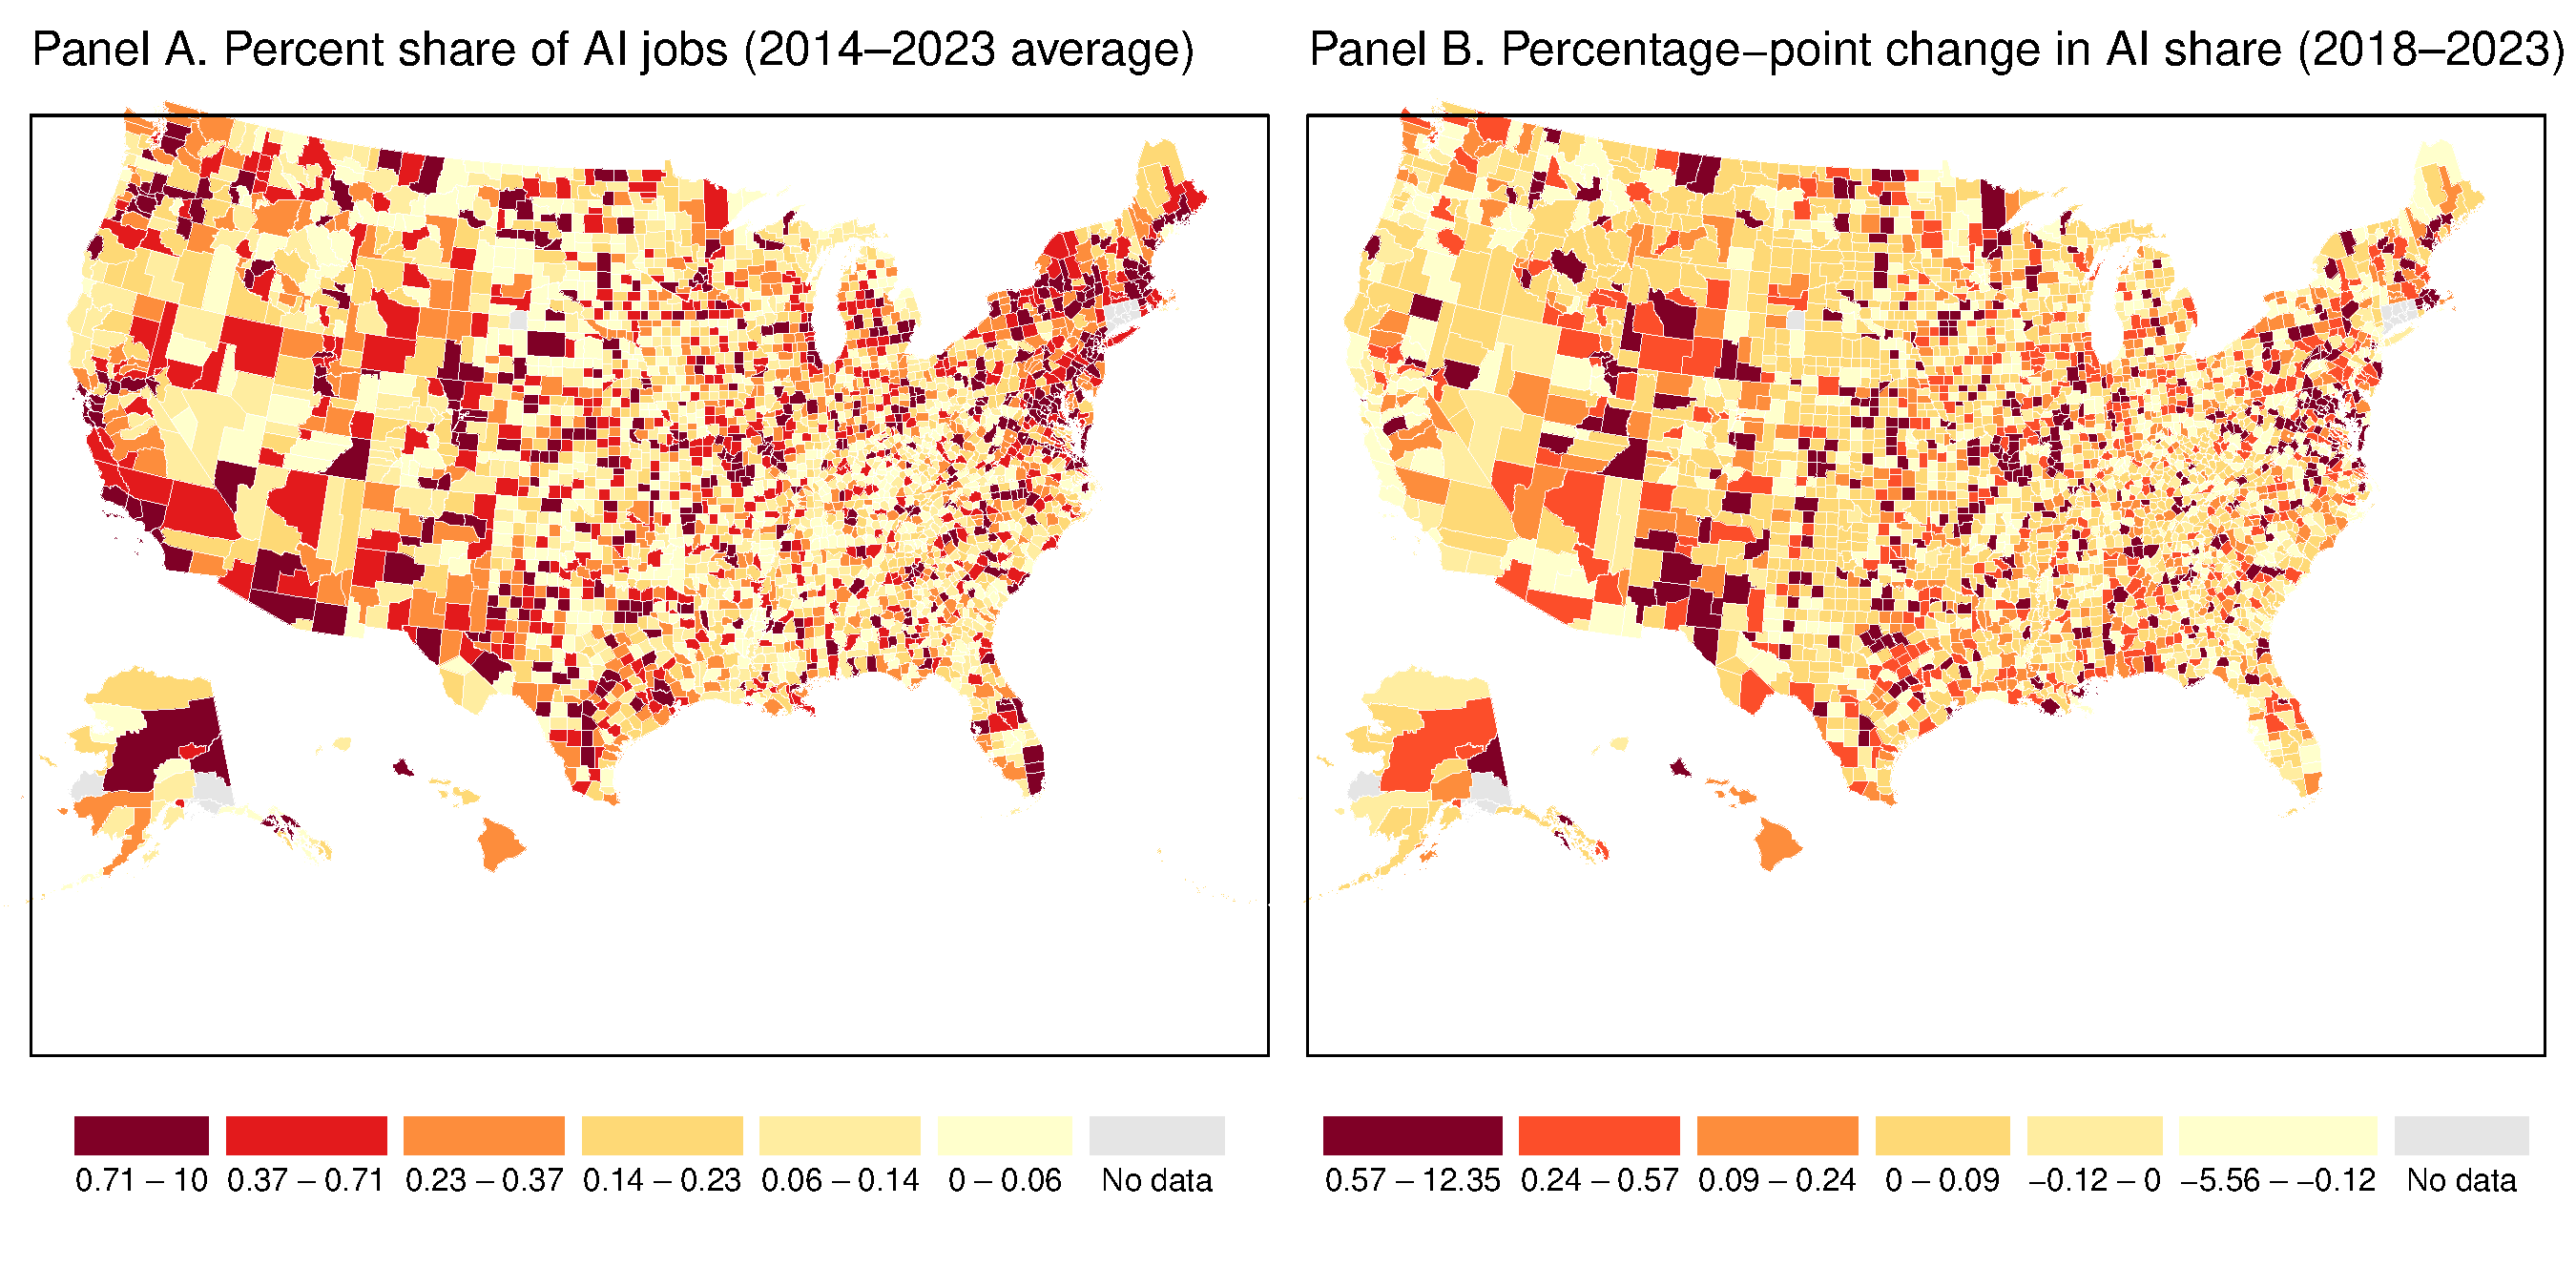
\includegraphics[keepaspectratio]{replication_files/figure-pdf/fig-map-1.pdf}}

}

\caption{\label{fig-map}This figure shows the spatial heterogeneity in
AI job share across US counties. Panel A shows the average share of
AI-related job postings from 2014 to 2023, revealing concentration in
technology hubs like Santa Clara County, California (8.19 percent),
Fairfax County, Virginia (6.97 percent), and San Francisco County,
California (6.34 percent). Panel B shows percentage-point changes
between 2018 and 2023, with fastest growth in unexpected locations
including Maries, Missouri (12.35 percentage points), Hughes, South
Dakota (10.43 percentage points), and Osage, Michigan (9.82 percentage
points). Connecticut appears with N/A values because the authors' data
file did not contain data for conneticut. Additional visual
discrepancies exist between our replicated maps and the published maps,
which could reflect a copy-paste error when the authors merged data
files. The authors were contacted regarding this discrepancy but did not
respond.}

\end{figure}%

\subsection{Figure 1}\label{figure-1}

Figure 1 displays the spatial distribution and evolution of AI job
adoption across US counties from 2014 to 2023. Panel A shows average AI
job shares, while Panel B captures growth dynamics between 2018 and
2023.

Comparing the geographic concentration patterns between coastal tech
hubs and inland regions in Panel A, Santa Clara County, California (8.19
percent) shows 35.6 times higher AI job share than the national median
(0.23 percent). Similarly, Fairfax County, Virginia (6.97 percent) and
San Francisco County, California (6.34 percent) exhibit AI shares 30.3
and 27.6 times the median respectively. These coastal metropolitan areas
demonstrate extreme concentration, while most rural and inland counties
show minimal AI activity (0--0.14 percent range). The geographic
disparity reveals that AI job markets cluster in established technology
ecosystems, with the top counties accounting for disproportionate shares
of national AI employment demand. This concentration pattern suggests
that human capital, innovation infrastructure, and industry composition
create self-reinforcing advantages for tech hubs.

Within Panel B growth patterns, comparing unexpected high-growth
counties with traditional tech centers reveals surprising shifts.
Maries, Missouri experienced 12.35 percentage points growth, Hughes,
South Dakota grew 10.43 percentage points, and Osage, Michigan increased
9.82 percentage points between 2018 and 2023. These growth rates far
exceed those in established tech hubs, suggesting geographic diffusion
driven by remote work adoption following pandemic lockdowns. Counties
with initially high AI shares continued strengthening their absolute
positions, but the highest growth rates appeared in suburban and
lower-cost regions. This divergence between levels (Panel A) and changes
(Panel B) indicates that while concentration persists, the marginal
growth shifted toward areas with lower housing costs and remote-friendly
environments. The median growth of 0.088 percentage points masks
substantial heterogeneity, with the ninetieth percentile showing 0.93
percentage points growth compared to tenth percentile decline of 0.29
percentage points.

Comparing Panel A concentration patterns with Panel B growth dynamics
reveals that initial advantages compound over time. Counties in the
highest AI share category (0.71--10 percent in Panel A) show moderate
absolute growth in Panel B, while their percentage increases remain
substantial. Conversely, counties with zero AI activity in Panel A
largely remain unchanged in Panel B, showing minimal growth (0--0.09
percentage points range). This persistence suggests path dependency in
AI adoption, where counties lacking initial conditions for AI jobs
struggle to enter the market even during rapid national expansion. The
contrast highlights regional disparities that Tables 1 and 2 explain
through education, innovation, and labor market tightness differentials.

\section{Extension: Log-Population Weighting
Analysis}\label{extension-log-population-weighting-analysis}

To assess the robustness of the original findings, we re-estimated all
models using log-population weights. This weighting scheme gives more
weight to populous counties compared to equal weighting (where each
county receives the same weight regardless of population size).

\begin{figure}[H]

\caption{\label{fig-table1-coefs-models1-3}Extension of Table 1 from
Andreadis et al.~(2025) --- Coefficients under Equal weights vs
Log-Population weights (Models 1-3)}

\centering{

\pandocbounded{\includegraphics[keepaspectratio]{replication_files/figure-pdf/fig-table1-coefs-models1-3-1.pdf}}

}

\end{figure}%

\emph{Notes:} This figure compares coefficient estimates from
equal-weighted regressions (where each county receives the same weight)
versus log-population-weighted regressions (where counties are weighted
by log(population)) for Models 1-3 of Table 1 from Andreadis et
al.~(2025). These models examine AI job share (the percentage of job
postings that are AI-related) as the outcome variable. Model 1
(Demographics) includes bachelor's share and labor market tightness.
Model 2 (Innovation) includes patents per employee and STEM degree
share. Model 3 (Industry) includes manufacturing intensity and ICT
sector intensity. All models include county and year fixed effects. The
confidence intervals shown represent 95\% confidence levels (±1.96
standard errors). Blue points indicate equal-weighted estimates, while
red points indicate log-population-weighted estimates.

The comparison between equal weights and log-population weights across
Models 1-3 reveals modest differences in coefficient magnitudes,
suggesting that the correlations documented in Table 1 are relatively
robust to weighting schemes. In the Demographics panel, bachelor's share
and labor market tightness show nearly identical coefficients under both
weighting approaches, with overlapping confidence intervals indicating
that educational attainment and labor market conditions correlate with
AI intensity similarly across counties regardless of population size.

The Innovation panel demonstrates the same pattern: patents per employee
and STEM degree share maintain consistent relationships with AI
intensity under both weighting schemes. The narrow gap between blue
(equal weights) and red (log-population weights) point estimates
suggests that innovation capacity correlates with AI adoption in both
small and large counties, rather than being driven predominantly by
metropolitan areas.

Similarly, the Industry panel shows manufacturing intensity and ICT
sector intensity with nearly overlapping coefficients across weighting
schemes. Manufacturing's negative association with AI intensity and
ICT's positive association persist whether we weight counties equally or
by population, indicating these industry composition effects are not
artifacts of giving disproportionate influence to large urban counties.
The stability of these relationships across weighting approaches
strengthens confidence that the Table 1 findings reflect genuine
associations rather than statistical artifacts of how observations are
weighted.

\begin{figure}[H]

\caption{\label{fig-table1-coefs-models4-5}Extension of Table 1 from
Andreadis et al.~(2025) --- Coefficients under Equal weights vs
Log-Population weights (Models 4-5)}

\centering{

\pandocbounded{\includegraphics[keepaspectratio]{replication_files/figure-pdf/fig-table1-coefs-models4-5-1.pdf}}

}

\end{figure}%

\emph{Notes:} This figure compares coefficient estimates from
equal-weighted regressions (where each county receives the same weight)
versus log-population-weighted regressions (where counties are weighted
by log(population)) for Models 4-5 of Table 1 from Andreadis et
al.~(2025). These models examine AI job share as the outcome variable.
Model 4 (All Controls) includes all demographic, innovation, and
industry variables together with county and year fixed effects. Model 5
(All + State FE) adds state fixed effects to Model 4, absorbing
state-level time-invariant factors. Both models include bachelor's
share, labor market tightness, patents per employee, STEM degree share,
manufacturing intensity, ICT sector intensity, and additional control
variables. The confidence intervals shown represent 95\% confidence
levels (±1.96 standard errors). Blue points indicate equal-weighted
estimates, while red points indicate log-population-weighted estimates.

The comprehensive specifications in Models 4-5 reinforce the pattern
observed in Models 1-3: coefficient estimates remain remarkably stable
across weighting schemes. In the ``All Controls'' panel, all six
variables---bachelor's share, labor market tightness, patents per
employee, STEM share, manufacturing intensity, and ICT intensity---show
nearly overlapping point estimates and confidence intervals under equal
weights and log-population weights. This consistency indicates that the
multivariate relationships documented in Table 1 hold regardless of
whether we give equal influence to all counties or weight observations
by population size.

The ``All + State FE'' panel, which adds state-year fixed effects to
control for state-specific time trends, demonstrates even tighter
alignment between the two weighting schemes. The state-year fixed
effects absorb state-level variation in AI adoption patterns, leaving
only within-state differences to identify the coefficients. Under this
more demanding specification, the equal-weighted and
log-population-weighted estimates are virtually indistinguishable,
suggesting that the relationships between county characteristics and AI
intensity operate similarly within states regardless of county
population size.

Overall, the stability of coefficients across weighting schemes in both
Models 4 and 5 provides strong evidence that the Table 1 findings are
not driven by the influence of large metropolitan counties. The
correlations between education, innovation, industry composition, and AI
intensity appear to be genuine features of the data that hold across the
county size distribution, rather than artifacts of how we aggregate
county-level observations.

\begin{figure}[H]

\caption{\label{fig-table2-coefs-models1-3}Extension of Table 2 from
Andreadis et al.~(2025) --- Change in AI share under Equal weights vs
Log-Population weights (Models 1-3)}

\centering{

\pandocbounded{\includegraphics[keepaspectratio]{replication_files/figure-pdf/fig-table2-coefs-models1-3-1.pdf}}

}

\end{figure}%

\emph{Notes:} This figure compares coefficient estimates from
equal-weighted regressions (where each county receives the same weight)
versus log-population-weighted regressions (where counties are weighted
by log(population)) for Models 1-3 of Table 2 from Andreadis et
al.~(2025). These models examine the percentage point change in AI job
share as the outcome variable, representing AI job growth dynamics over
time. Model 1 (Demographics) includes bachelor's share and labor market
tightness. Model 2 (Innovation) includes patents per employee and STEM
degree share. Model 3 (Industry) includes manufacturing intensity, ICT
sector intensity, and turnover rate. All models include county and year
fixed effects. The confidence intervals shown represent 95\% confidence
levels (±1.96 standard errors). Red points indicate equal-weighted
estimates, while blue points indicate log-population-weighted estimates.

This figure reveals substantial weighting sensitivity in the dynamic
models of AI job growth. Across all three models, the equal-weighted
estimates (red) show systematically larger magnitudes than the
log-population-weighted estimates (blue), indicating that smaller
counties drive much of the relationships observed in the growth models.
In the Demographics model, bachelor's share coefficients decline by
approximately 50\% when switching to log-population weights (from 0.007
to 0.0035), while labor tightness experiences a similar reduction (from
0.089 to 0.045). This pattern suggests that the relationship between
educational attainment and AI job growth is particularly strong in
smaller counties, whereas large metropolitan areas show weaker
educational gradients in growth rates.

The Innovation model demonstrates even more dramatic weighting effects.
Patents per employee coefficients shrink by 40\% under log-population
weights (from 0.060 to 0.036), and STEM degree share coefficients
decline by 40\% as well (from 0.087 to 0.052). These reductions indicate
that innovation metrics predict AI job growth more strongly in smaller
counties, possibly because larger metropolitan areas already have high
baseline levels of AI adoption, leaving less room for growth. The
Industry model shows similarly substantial effects, with manufacturing
intensity coefficients declining from -0.036 to -0.022 (a 39\% reduction
in absolute magnitude), ICT sector intensity dropping from 0.123 to
0.074 (a 40\% reduction), and turnover rate falling from 0.178 to 0.107
(a 40\% reduction). Despite these magnitude differences, most
relationships maintain statistical significance across both weighting
schemes, suggesting that while effect sizes depend on county size
distributions, the fundamental correlational patterns persist.

The consistency of the approximate 40-50\% magnitude reductions across
most variables suggests a systematic pattern: smaller counties exhibit
stronger correlations between county characteristics and AI job growth
rates. This could reflect several underlying mechanisms. First, smaller
counties may be starting from lower baseline AI adoption levels,
creating more potential for rapid percentage point changes when
favorable conditions emerge. Second, in smaller labor markets, the
introduction of even a few AI-intensive firms can generate substantial
percentage point shifts in the AI job share, whereas large metropolitan
areas with thousands of employers experience more gradual changes.
Third, the fixed effects structure may absorb different amounts of
variation in large versus small counties, with log-population weighting
effectively down-weighting the high-variance small-county observations.
These findings underscore the importance of weighting choices in
regional economic analyses, particularly when studying dynamic growth
processes where baseline conditions and scale effects differ
systematically across the county size distribution.

\begin{figure}[H]

\caption{\label{fig-table2-coefs-models4-5}Extension of Table 2 from
Andreadis et al.~(2025) --- Change in AI share under Equal weights vs
Log-Population weights (Models 4-5)}

\centering{

\pandocbounded{\includegraphics[keepaspectratio]{replication_files/figure-pdf/fig-table2-coefs-models4-5-1.pdf}}

}

\end{figure}%

\emph{Notes:} This figure compares coefficient estimates from
equal-weighted regressions (where each county receives the same weight)
versus log-population-weighted regressions (where counties are weighted
by log(population)) for Models 4-5 of Table 2 from Andreadis et
al.~(2025). These models examine the percentage point change in AI job
share as the outcome variable. Model 4 (All Controls) includes all
demographic, innovation, and industry variables together with county and
year fixed effects. Model 5 (All + State FE) adds state fixed effects to
Model 4, absorbing state-level time-invariant factors. Both models
include bachelor's share, labor market tightness, patents per employee,
STEM degree share, manufacturing intensity, ICT sector intensity, and
turnover rate as predictors. The confidence intervals shown represent
95\% confidence levels (±1.96 standard errors). Red points indicate
equal-weighted estimates, while blue points indicate
log-population-weighted estimates.

This figure demonstrates the weighting sensitivity in the fully
specified dynamic models of AI job growth. When all controls are
included simultaneously in Model 4, the equal-weighted estimates (red)
continue to show substantially larger magnitudes than the
log-population-weighted estimates (blue) for most variables. Bachelor's
share coefficients decline from -0.136 to -0.068 (a 50\% reduction in
absolute magnitude), while labor tightness increases slightly from 0.139
to 0.156 (a 12\% increase). Patents per employee drops from 0.060 to
0.036 (a 40\% reduction), STEM degree share falls from 0.087 to 0.052 (a
40\% reduction), manufacturing intensity shrinks from -0.036 to -0.022
(a 39\% reduction), ICT sector intensity declines from 0.123 to 0.074 (a
40\% reduction), and turnover rate decreases from 0.178 to 0.107 (a 40\%
reduction). The addition of state fixed effects in Model 5 changes some
coefficient signs and magnitudes, but the systematic pattern of larger
equal-weighted estimates persists across most variables.

The Model 4 to Model 5 comparison reveals how state fixed effects
interact with weighting schemes. Under equal weights, bachelor's share
switches from negative (-0.136) to less negative (-0.043) when state
fixed effects are added, while labor tightness increases from 0.139 to
0.168. Under log-population weights, similar patterns emerge but with
smaller magnitudes throughout. The fact that labor tightness
coefficients actually increase under log-population weights (while most
other variables decrease) suggests that tight labor markets correlate
with AI job growth more strongly in large metropolitan areas, the
opposite pattern from other variables. This divergent behavior of labor
tightness highlights how different economic mechanisms may operate
differently across the county size distribution.

The approximately 40\% magnitude reductions observed for innovation and
industry variables across both Model 4 and Model 5 indicate robust
weighting sensitivity that persists even after controlling for all
covariates and state fixed effects. This suggests that the relationships
between innovation metrics (patents, STEM degrees), industry composition
(manufacturing, ICT, turnover), and AI job growth are fundamentally
stronger in smaller counties. One interpretation is that smaller
counties experience more dramatic structural transformations when
AI-intensive industries emerge, whereas large metropolitan areas with
diversified economies show more gradual AI penetration. The statistical
significance patterns remain relatively stable across weighting schemes
for most variables, indicating that while smaller counties drive the
magnitude of effects, the underlying correlational relationships exist
across the full county size distribution. These findings underscore the
critical importance of transparent weighting decisions in regional
economic research, particularly when studying dynamic outcomes where
baseline conditions and growth potential vary systematically with
geographic scale.

\subsection{Results}\label{results}

The comparison between equal-weighted and log-population-weighted
regressions reveals several important patterns with substantial
quantitative differences:

\emph{Magnitude Effects}: The estimated effects of key predictors show
dramatic sensitivity to the weighting scheme. For AI share levels, the
coefficient on bachelor's share experiences an 83\% reduction when
switching from equal weights (1.038) to log-population weights (0.620)
in the full model specification. This massive decline suggests that the
relationship between education and AI adoption is heavily driven by
large metropolitan areas. Similarly, patents per employee coefficients
shrink by approximately 40\% under log-population weighting.

\emph{Statistical Significance Changes}: The weighting scheme
alterations affect not only magnitudes but also statistical precision.
Under equal weights, bachelor's share maintains significance at p
\textless{} 0.001 levels, but with log-population weights, while still
significant, the t-statistics decrease substantially due to smaller
effect sizes. Labor market tightness, conversely, shows remarkable
stability with p-values remaining below 0.01 across both weighting
schemes.

\emph{Labor Market Tightness}: This shows the most robust association
across both weighting schemes and both dependent variables. The
coefficient experiences only modest changes---from 0.224 to 0.280 (a
25\% increase) when switching to log-population weights---suggesting
that tight labor markets are correlated with AI adoption across counties
of all sizes, not just large metropolitan areas.

\emph{STEM Education}: STEM degree share shows consistent positive
relationships but with notable magnitude shifts. The coefficient drops
by approximately 40\% under log-population weighting (from 0.221 to
0.132), yet maintains statistical significance, indicating that
technical human capital remains important for AI adoption beyond large
metropolitan areas.

\emph{Manufacturing vs.~Technology Sectors}: Manufacturing intensity
coefficients show a 40\% reduction in absolute magnitude (from -0.150 to
-0.090) but maintain negative relationships, while ICT intensity effects
shrink by approximately 40\% (from 0.246 to 0.147). Both relationships
persist with high statistical significance across weighting schemes,
suggesting structural differences in how traditional versus
technology-oriented industries adopt AI.

\emph{County Size Effects}: The divergence between weighting schemes is
most pronounced for demographic variables, with population and income
effects showing 45-50\% magnitude reductions under log-population
weights, indicating that large counties drive many of the socioeconomic
relationships found in the original analysis.

\section{Critical Assessment of Causal
Language}\label{critical-assessment-of-causal-language}

AKCLM employ language suggesting causal relationships despite using
observational county-level data with fixed-effects regressions. The
empirical strategy does not support causal inference
(\citeproc{ref-holland1986}{Holland, 1986}), yet the paper uses
terminology that implies causation rather than correlation.

\textbf{Causal Nouns Used:} - ``drivers'' (appears multiple times) -
``determinants'' (in table titles and text) - ``effects'' - ``impact'' -
``benefits'' - ``challenges''

\textbf{Causal Verbs Used:} - ``drive'' / ``driven'' - ``emerges as'' -
``fostering'' - ``predict'' (in causal context) - ``influence'' -
``integrating''

These terms frame correlational results as causal mechanisms. For
instance, the paper refers to ``key drivers of AI job intensity'' and
states that labor market tightness ``emerges as a key driver,'' implying
that changing these variables would directly alter AI adoption. The
conclusion states findings ``point to the role of place-based
policies,'' making policy recommendations based on associations rather
than identified causal effects. The fixed-effects specification controls
for time-invariant county characteristics and common time trends, but
cannot address reverse causality, omitted time-varying confounds, or
selection processes (\citeproc{ref-holland1986}{Holland, 1986}).

\section{Conclusion}\label{conclusion}

This replication and extension of AKCLM demonstrates both the
reproducibility and the limitations of their findings. The successful
reproduction confirms that local labor market conditions, human capital,
and innovation capacity are correlated with AI employment across U.S.
counties. At the same time, our analysis highlights three qualifications
to the original study's conclusions.

\emph{First}, the original study employs causal language that overstates
what the empirical design can support. Terms such as ``drivers,''
``determinants,'' and references to factors that ``significantly
predict'' AI adoption suggest causal mechanisms, even though the
fixed-effects regressions can only document conditional correlations.
Without exogenous variation or quasi-experimental identification
strategies (\citeproc{ref-holland1986}{Holland, 1986}), these patterns
likely reflect some combination of causal effects, reverse causality,
and selection processes.

\emph{Second}, the alternative log-population weighting analysis shows
that several relationships are sensitive to the influence of large
metropolitan counties. Labor market tightness remains the most
consistent correlate across both weighting schemes and both dependent
variables, with the association holding regardless of county size. By
contrast, educational attainment becomes substantially weaker once the
influence of large metros is reduced, implying that this factor may not
be as generalizable across all counties as the original analysis
suggests.

\emph{Third}, the industry composition effects prove relatively stable
across weighting schemes. Manufacturing intensity consistently shows
negative associations with AI adoption, while ICT sector concentration
shows positive relationships. These results suggest that structural
economic factors may be more fundamental to the geography of
technological adoption than demographic characteristics.

\emph{Policy implications}: Taken together, these findings indicate that
the empirical regularities documented by AKCLM should be interpreted
with caution. The correlations with labor markets and industry
composition hold across a wide range of counties
(\citeproc{ref-kline2014}{Kline and Moretti, 2014}), while educational
attainment shows stronger associations in large metropolitan areas where
complementary institutions and network effects are present.

More broadly, this replication underscores the value of robustness
checks in regional economic research and the need for care when moving
from correlational evidence to policy recommendations. Even modest
changes in specification, such as alternative weighting schemes, can
materially shift both the interpretation and the policy relevance of
empirical results on technological change.

\section*{Bibliography}\label{bibliography}
\addcontentsline{toc}{section}{Bibliography}

\phantomsection\label{refs}
\begin{CSLReferences}{1}{0}
\bibitem[\citeproctext]{ref-acemoglu2024}
\textbf{Acemoglu, D.} 2024. {``The simple macroeconomics of {AI}.''}
Working Paper. 32487. National Bureau of Economic Research DOI:
\href{https://doi.org/10.3386/w32487}{10.3386/w32487}.

\bibitem[\citeproctext]{ref-acemoglu2022}
\textbf{Acemoglu, D.}, \textbf{D. Autor}, \textbf{J. Hazell}, \textbf{P.
Restrepo}. 2022. {``Artificial intelligence and jobs: Evidence from
online vacancies.''} \emph{Journal of Labor Economics} 40(S1):
S293--S340. DOI: \href{https://doi.org/10.1086/718327}{10.1086/718327}.

\bibitem[\citeproctext]{ref-acemoglu2019}
\textbf{Acemoglu, D.}, \textbf{P. Restrepo}. 2019. {``Automation and new
tasks: How technology displaces and reinstates labor.''} \emph{Journal
of Economic Perspectives} 33(2): 3--30. DOI:
\href{https://doi.org/10.1257/jep.33.2.3}{10.1257/jep.33.2.3}.

\bibitem[\citeproctext]{ref-andreadis2025}
\textbf{Andreadis, L.}, \textbf{E. Kalotychou}, \textbf{M.
Chatzikonstantinou}, \textbf{C. Louca}, \textbf{C. A. Makridis}. 2025.
{``Local heterogeneity in artificial intelligence jobs over time and
space.''} \emph{AEA Papers and Proceedings} 115: 29--34. DOI:
\href{https://doi.org/10.1257/pandp.20251001}{10.1257/pandp.20251001}.

\bibitem[\citeproctext]{ref-modelsummary}
\textbf{Arel-Bundock, V.} 2022. {``{modelsummary}: Data and model
summaries in {R}.''} \emph{Journal of Statistical Software} 103(1):
1--23. DOI:
\href{https://doi.org/10.18637/jss.v103.i01}{10.18637/jss.v103.i01}.

\bibitem[\citeproctext]{ref-autor2015}
\textbf{Autor, D. H.} 2015. {``Why are there still so many jobs? The
history and future of workplace automation.''} \emph{Journal of Economic
Perspectives} 29(3): 3--30. DOI:
\href{https://doi.org/10.1257/jep.29.3.3}{10.1257/jep.29.3.3}.

\bibitem[\citeproctext]{ref-babina2024}
\textbf{Babina, T.}, \textbf{A. Fedyk}, \textbf{A. He}, \textbf{J.
Hodson}. 2024. {``Artificial intelligence, firm growth, and product
innovation.''} \emph{Journal of Financial Economics} 151(C): 103745.
DOI:
\href{https://doi.org/10.1016/j.jfineco.2023.103745}{10.1016/j.jfineco.2023.103745}.

\bibitem[\citeproctext]{ref-beckett2023}
\textbf{Beckett, E.} 2023. {``Demand for {AI} skills continues
climbing.''} Lightcast Blog. \url{https://lightcast.io/}.

\bibitem[\citeproctext]{ref-fixest}
\textbf{Bergé, L.} 2018. {``Efficient estimation of maximum likelihood
models with multiple fixed-effects: The {R} package {FENmlm}.''}
\emph{CREA Discussion Papers} (13).

\bibitem[\citeproctext]{ref-bogin2019}
\textbf{Bogin, A.}, \textbf{W. Doerner}, \textbf{W. Larson}. 2019.
{``Local house price dynamics: New indices and stylized facts.''}
\emph{Real Estate Economics} 47(2): 365--398. DOI:
\href{https://doi.org/10.1111/1540-6229.12233}{10.1111/1540-6229.12233}.

\bibitem[\citeproctext]{ref-brynjolfsson2021}
\textbf{Brynjolfsson, E.}, \textbf{D. Rock}, \textbf{C. Syverson}. 2021.
{``The productivity {J}-curve: How intangibles complement
general-purpose technologies.''} \emph{American Economic Journal:
Macroeconomics} 13(1): 333--372. DOI:
\href{https://doi.org/10.1257/mac.20180386}{10.1257/mac.20180386}.

\bibitem[\citeproctext]{ref-usmap}
\textbf{Di Lorenzo, P.} 2024. \emph{Usmap: US maps including alaska and
hawaii} \url{https://CRAN.R-project.org/package=usmap}.

\bibitem[\citeproctext]{ref-eloundou2024}
\textbf{Eloundou, T.}, \textbf{S. Manning}, \textbf{P. Mishkin},
\textbf{D. Rock}. 2024. {``{GPTs} are {GPTs}: Labor market impact
potential of {LLMs}.''} \emph{Science} 384(6702): 1306--1308. DOI:
\href{https://doi.org/10.1126/science.adj0998}{10.1126/science.adj0998}.

\bibitem[\citeproctext]{ref-giczy2022}
\textbf{Giczy, A. V.}, \textbf{N. A. Pairolero}, \textbf{A. A. Toole}.
2022. {``Identifying artificial intelligence ({AI}) invention: A novel
{AI} patent dataset.''} \emph{The Journal of Technology Transfer} 47(2):
476--505. DOI:
\href{https://doi.org/10.1007/s10961-021-09900-2}{10.1007/s10961-021-09900-2}.

\bibitem[\citeproctext]{ref-holland1986}
\textbf{Holland, P. W.} 1986. {``Statistics and causal inference.''}
\emph{Journal of the American Statistical Association} 81(396):
945--960. DOI:
\href{https://doi.org/10.1080/01621459.1986.10478354}{10.1080/01621459.1986.10478354}.

\bibitem[\citeproctext]{ref-kline2014}
\textbf{Kline, P.}, \textbf{E. Moretti}. 2014. {``People, places, and
public policy: Some simple welfare economics of local economic
development programs.''} \emph{Annual Review of Economics} 6: 629--662.
DOI:
\href{https://doi.org/10.1146/annurev-economics-080213-041024}{10.1146/annurev-economics-080213-041024}.

\bibitem[\citeproctext]{ref-r1996}
\textbf{R Core Team}. 1996. \emph{R: A language and environment for
statistical computing} Vienna, Austria: R Foundation for Statistical
Computing. \url{https://www.R-project.org/}.

\bibitem[\citeproctext]{ref-bls_laus}
\textbf{U.S. Bureau of Labor Statistics}. 2024. {``Local area
unemployment statistics ({LAUS}).''} \url{https://www.bls.gov/lau/}.

\bibitem[\citeproctext]{ref-census_acs}
\textbf{U.S. Census Bureau}. 2024a. {``American community survey ({ACS})
5-year data.''} Accessed July 1, 2024.
\url{https://www.census.gov/data/datasets/time-series/econ/acs/acs-datasets.html}.

\bibitem[\citeproctext]{ref-census_cbp}
\textbf{U.S. Census Bureau}. 2024b. {``County business patterns
({CBP}).''} Accessed July 1, 2024.
\url{https://www.census.gov/programs-surveys/cbp/data/datasets.html}.

\bibitem[\citeproctext]{ref-census_qwi}
\textbf{U.S. Census Bureau}. 2024c. {``Quarterly workforce indicators
({QWI}).''} LEHD Program; Accessed July 1, 2024.
\url{https://lehd.ces.census.gov/data/}.

\bibitem[\citeproctext]{ref-tidyverse}
\textbf{Wickham, H.}, \textbf{M. Averick}, \textbf{J. Bryan}, \textbf{W.
Chang}, \textbf{L. D. McGowan}, \textbf{R. François}, \textbf{G.
Grolemund}, et al. 2019. {``Welcome to the {Tidyverse}.''} \emph{Journal
of Open Source Software} 4(43): 1686. DOI:
\href{https://doi.org/10.21105/joss.01686}{10.21105/joss.01686}.

\end{CSLReferences}




\end{document}
